\documentclass[12pt]{article}
\usepackage{graphicx}
\begin{document}

\section*{High-level description of the algorithm}

In the following sections, we discuss how the abstract version algorithm works and explain its requirements for implementation. The general idea is to have processes agree on the linearization and then respond fast from the history.

\subsection*{Tree specs}
\begin{figure}[hbt]
  \center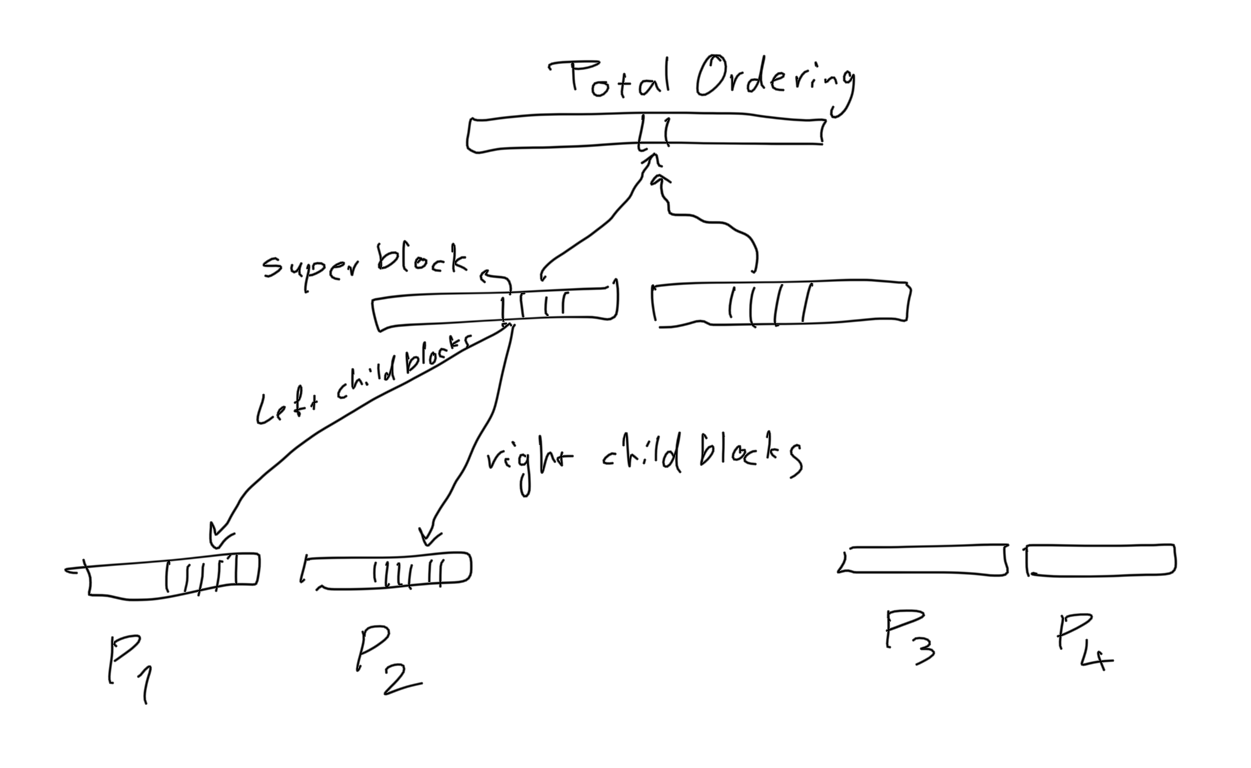
\includegraphics[width=4in]{pics/tree}
  \caption{An example of a linearizable execution. Both could take effect first since ENQ(A), and ENQ(B) are concurrent.}
\end{figure}
A block is an ordering on some operations. Note that it does not necessarily contain the operations. Each node contains an ordering of blocks appended to it. Process $p_i$ adds $op$ to a block in its node and propagates it to the root, which stores the total ordering.

\paragraph{Propagate(node n):}
\begin{enumerate}
  \item Create a block from $n$'s children's blocks which are not already in $n$
  \item Append the block to $n$
  \item If 2 was not successful, do 1-2 one more time
\end{enumerate}

\paragraph{Requirements}
Creating a block takes less than $O(\log p)$ steps. If some processes try to append their block into node $n$ simultaneously, at least one of them succeeds.

\paragraph{Linearization}
Operations are linearized when they are added to the root. The operations in a block are linearized as the block's ordering. Methods $Get(i)$ and $Index(op)$ give us information about the linearization.

\paragraph{Get(i):} gets the $i$th operation in the total ordering
\begin{enumerate}
  \item $B$= find the block containing $i$th in the root 
\marginpar{\begin{flushleft}\scriptsize{$\log \#ops$ steps}\end{flushleft}}
  \item Get(B, i-pre(B), root) 
\marginpar{\begin{flushleft}\scriptsize{pre(B) is \#operations before B}\end{flushleft}}
\end{enumerate}

\paragraph{Get(B,i,n):} gets the $i$th operation in block B in node n
\begin{enumerate}
  \item $SB$= find the subblock of B containing $i$th op
\marginpar{\begin{flushleft}\scriptsize{$\log p$ steps}\end{flushleft}}
  \item Get(SB, i-pre(SB), B's node)
\end{enumerate}

\paragraph{Requirements} Each level of Get() takes $\log p$ steps, and there are $\log p$ levels. So Get may take $O(\log \#ops + \log^2 p)$. In the following, we discuss that Get is going to be called on the current values of the Queue, so it is going to be $\log Q$.

\paragraph{Index(op):} Where is the position of propagated operation op? It will be done by recursively calling Index(n,b,i) in the path from a leaf up to the root.

\paragraph{Index(n,B,i):}
\begin{enumerate}
  \item $SB$= find the block in n's parent that contains ith op in block B of node n
\marginpar{\begin{flushleft}\scriptsize{$\log p$ steps}\end{flushleft}}
  \item Index(n,B,i+pre(SB))
\end{enumerate}

\paragraph{Requirements} find the superblock of a block in $\log p$ steps

\section*{Transform to a Queue} We are going to augment the root blocks to find out which index is the head of Queue while a Dequeue is linearized.

\paragraph{Enqueue(v):} Add ENQ(v) to the tree
\paragraph{Dequeue():}
\begin{enumerate}
  \item Add DEQ() to the tree
  \item Index the DEQ() order
  \item Compute the index of the ENQ() which is the response of DEQ()
\marginpar{\begin{flushleft}\scriptsize{might be null}\end{flushleft}}
\item Get(i) and return the argument
\end{enumerate}

\paragraph{Requirements}
Augment root blocks so that 3 is fast. Get(i) takes $\log Q+ \log^2 p$.



\end{document}